\documentclass[tikz,border=4pt]{standalone}
\usepackage{amsmath,amssymb,bm,setspace}
\usepackage{tikz,pgfplots}
\pgfplotsset{compat=1.18}
\usetikzlibrary{arrows.meta,calc,positioning,decorations.pathreplacing}
\begin{document}
% Case-B rotational-stiffness comparison. The legend gives the measured
% measured angular-offset range across the three stiffness settings.
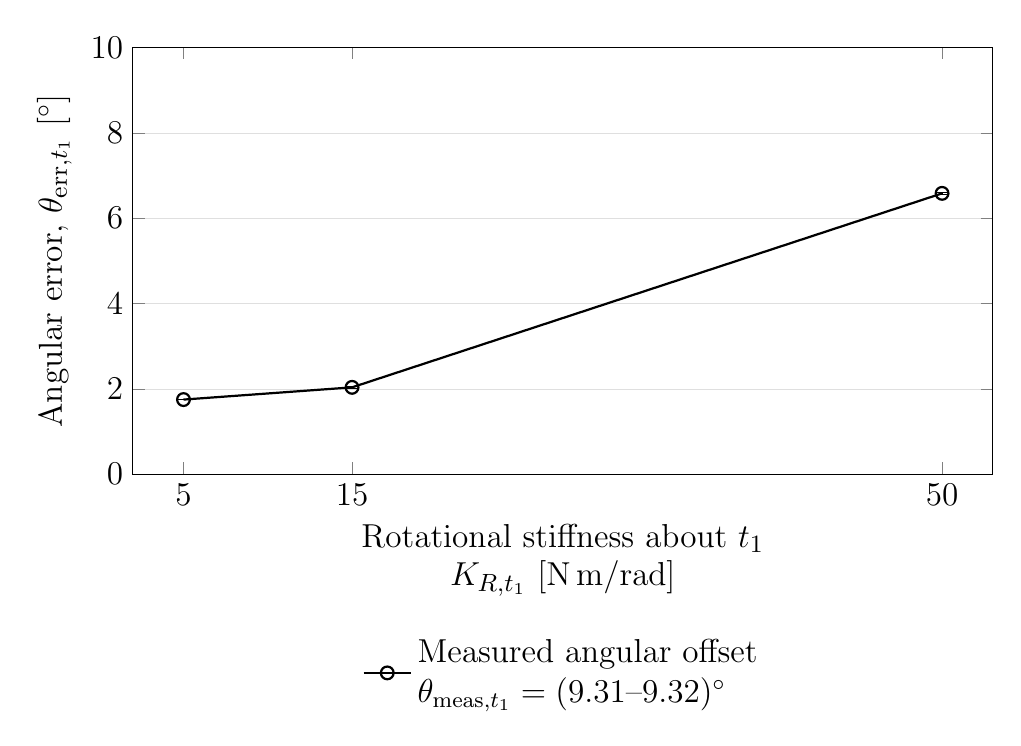
\begin{tikzpicture}
\begin{axis}[
    width=12.5cm, height=7.0cm,
    xmin=2, xmax=53, ymin=0, ymax=10,
    xtick={5,15,50},
    ytick={0,2,4,6,8,10},
    ymajorgrids=true, xmajorgrids=false,
    grid style={gray!25, very thin},
    tick label style={font=\fontsize{12}{14}\selectfont},
    label style={font=\fontsize{13}{15}\selectfont},
    xlabel={\shortstack{Rotational stiffness about $t_1$\\$K_{R,t_1}$ [N\,m/rad]}},
    ylabel={Angular error, \(\theta_{\mathrm{err},t_1}\) [\(^\circ\)]},
    legend style={font=\fontsize{12}{14}\selectfont, draw=none, fill=none,
                  cells={anchor=west}, at={(0.5,-0.36)}, anchor=north},
    every axis plot/.append style={thick, mark size=2.3pt},
  ]
\addplot[black, mark=o, mark options={fill=white},
         error bars/.cd, y dir=both, y explicit] coordinates {
  (5,1.750000000) +- (0,0.000000000)
  (15,2.036666667) +- (0,0.023094011)
  (50,6.583333333) +- (0,0.030550505)};
\addlegendentry{\shortstack[l]{Measured angular offset\\\(\theta_{\mathrm{meas},t_1}=(9.31\text{--}9.32)^\circ\)}}
\end{axis}
\end{tikzpicture}

\end{document}
